\documentclass{article}
\usepackage[utf8]{inputenc}
\usepackage[margin=1in]{geometry}
\usepackage{graphicx}
\usepackage{float}
\usepackage{caption}
\usepackage{hyperref}
\begin{document}
\title{PHY566 Group Project 1 Version B}
\author{Lingfei Zhao, Yuan Ji, Melissa Wu}
\maketitle

\begin{center}
\textit{\large Random Walk, Diffusion, and Mixing}\par
\end{center}
\bigskip
1. \textbf{2D Random Walk}\par
\smallskip
We simulate a random walker in 2 dimensions, taking steps of unit length in $\pm x$ or $\pm y$ on a discrete square lattice.\par
Let $n$ be the number of steps taken, $\langle x_{n} \rangle$ be the average $x$ displacement, $\langle (x_{n})^{2} \rangle$ be the average $x$ displacement squared, and $\langle r^{2} \rangle$ be the average total displacement squared. We plot $\langle x_{n} \rangle$, $\langle (x_{n})^{2} \rangle$, and $\langle r^{2} \rangle$ versus $n$ for up to $n = 100$ by averaging over at least $10^{4}$ different walks for each $n > 3$:\par
\begin{figure}[H]
\centering
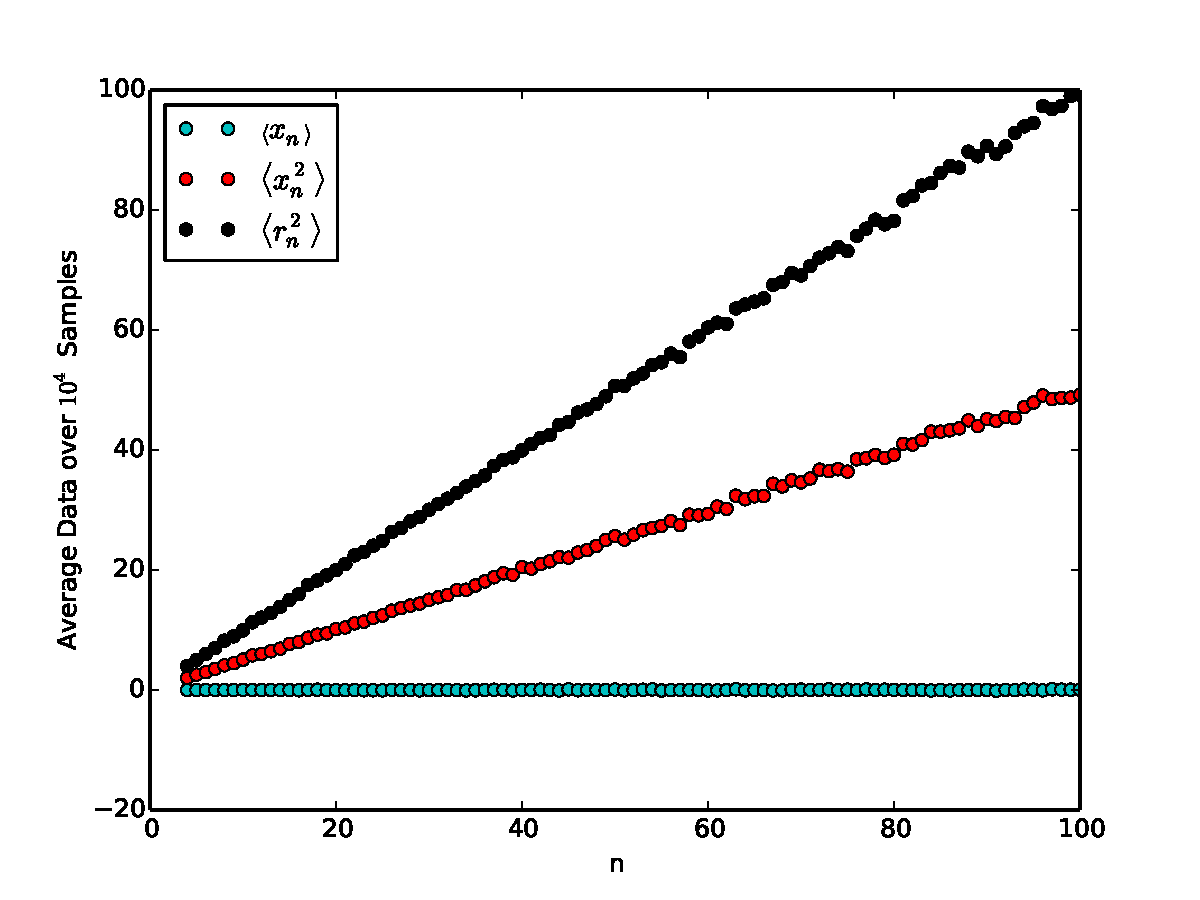
\includegraphics[width=10cm]{average.pdf}
\caption{Average of the $x$ displacement, $x^{2}$ displacement, and $r^{2}$ (total) displacement versus number of steps.}
\end{figure}
$\langle x_{n} \rangle$ is zero for all values of $n$, as expected: since the steps are random, we expect an equal number of steps in $+x$ as $-x$, averaging out to a net zero displacement from the origin. $\langle(x_{n})^{2} \rangle$ seems to follow a linear relationship with $n$ with a slope of $\frac{1}{2}$, i.e. $\langle(x_{n})^{2} \rangle \approx \frac{1}{2}n$. $\langle r^{2} \rangle$ seems to follow a linear relationship with $n$ as well, such that $\langle r^{2} \rangle \approx n$. Since $\langle r^{2} \rangle = 2Dn$, $D$ being the diffusion constant, we estimate $D \approx \frac{1}{2}$. This is expected as well, since the value of $\langle r^{2} \rangle$ can be calculated analytically to go to $n$, which would give an expected value of $D = \frac{1}{2}$.\par
\bigskip
\noindent 2. \textbf{Diffusion Equation}\par
\smallskip
We show analytically that the spatial expectation value of $\langle x(t)^{2} \rangle$ of the 1D Normal Distribution,

\begin{equation}
\rho(x,t) = \frac{1}{\sqrt{2\pi\sigma(t)^{2}}} \exp \bigg(-\frac{x^{2}}{2\sigma(t)^{2}}\bigg)
\end{equation}
equals $\sigma(t)^{2}$.\par
\noindent The expectation value of $\langle x(t)^{2} \rangle$ is defined as

\begin{equation}
\langle x(t)^{2} \rangle = \frac{1}{\sqrt{2\pi\sigma(t)^{2}}} \int_{-\infty}^{\infty} x^{2} \exp \bigg(-\frac{x^{2}}{2\sigma(t)^{2}}\bigg) dx
\label{eq:2}
\end{equation}
Let $y = x/\sqrt{2}\sigma(t)$. Then Equation \ref{eq:2} is just a Gaussian integral:
\begin{equation}
\langle x(t)^{2} \rangle = \frac{2\sigma(t)^2}{\sqrt{\pi}} \int_{-\infty}^{\infty} y^{2} \exp(-y^{2}) dy
\end{equation}
\begin{equation}
= \frac{2\sigma(t)^2}{\sqrt{\pi}} \bigg(\frac{\sqrt{\pi}}{2}\bigg)
\end{equation}
\begin{equation}
= \sigma(t)^{2}
\end{equation}
Now we want to solve the 1D diffusion equation using the finite difference form with a diffusion constant D = 2. We choose an initial density profile that is sharply peaked around $x = 0$, but plot multiple profiles at varying times $t$. We fit each density profile with the graph of a normal distribution to verify that the profiles correspond with the distribution. We note that at later times, the fit corresponds to a normal distribution with $\sigma(t) = \sqrt{2Dt}$.\par
\begin{figure}[H]
\centering
\captionsetup{justification=centering, margin=3.5cm}
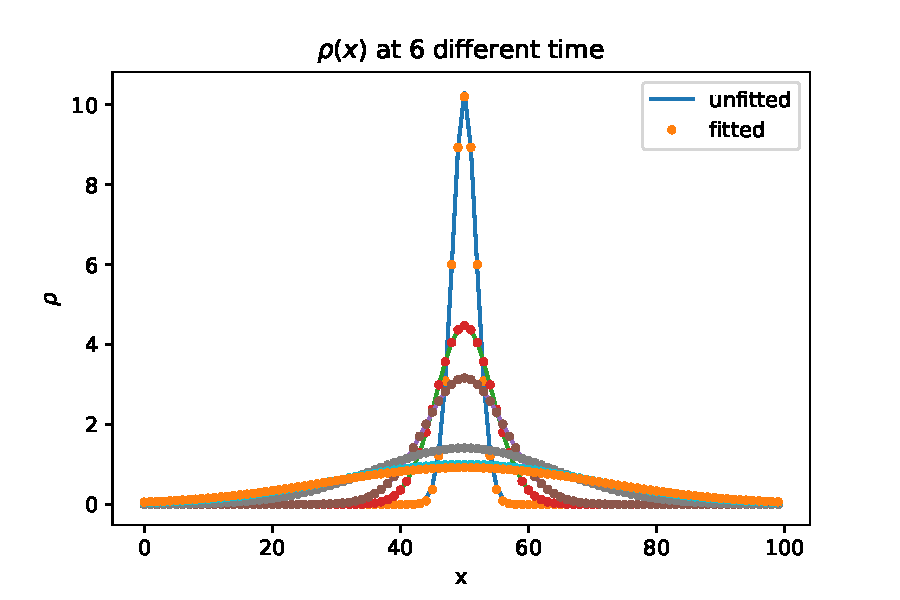
\includegraphics[width=10cm]{snapshots.pdf}
\caption{Density profiles of the 1D diffusion equation at various times, with fitted normal distributions overlayed.}
\end{figure}
\noindent As expected, although the initial density profile is sharply peaked, the profiles flatten out as time goes on, with middle two profiles at $t = 10 s$ and $t = 50 s$ most resembling a normal distribution. We note that the fitted distribution plots correspond nicely to our calculated profiles. To further verify our results, we also plot the parameters $\sigma(t)$ vs. $t$ and $\sigma^{2}(t)$ vs. $t$ to confirm that they follow the expected relationship $\sigma(t) = \sqrt{2Dt}$.\par
\begin{figure}[H]
\centering
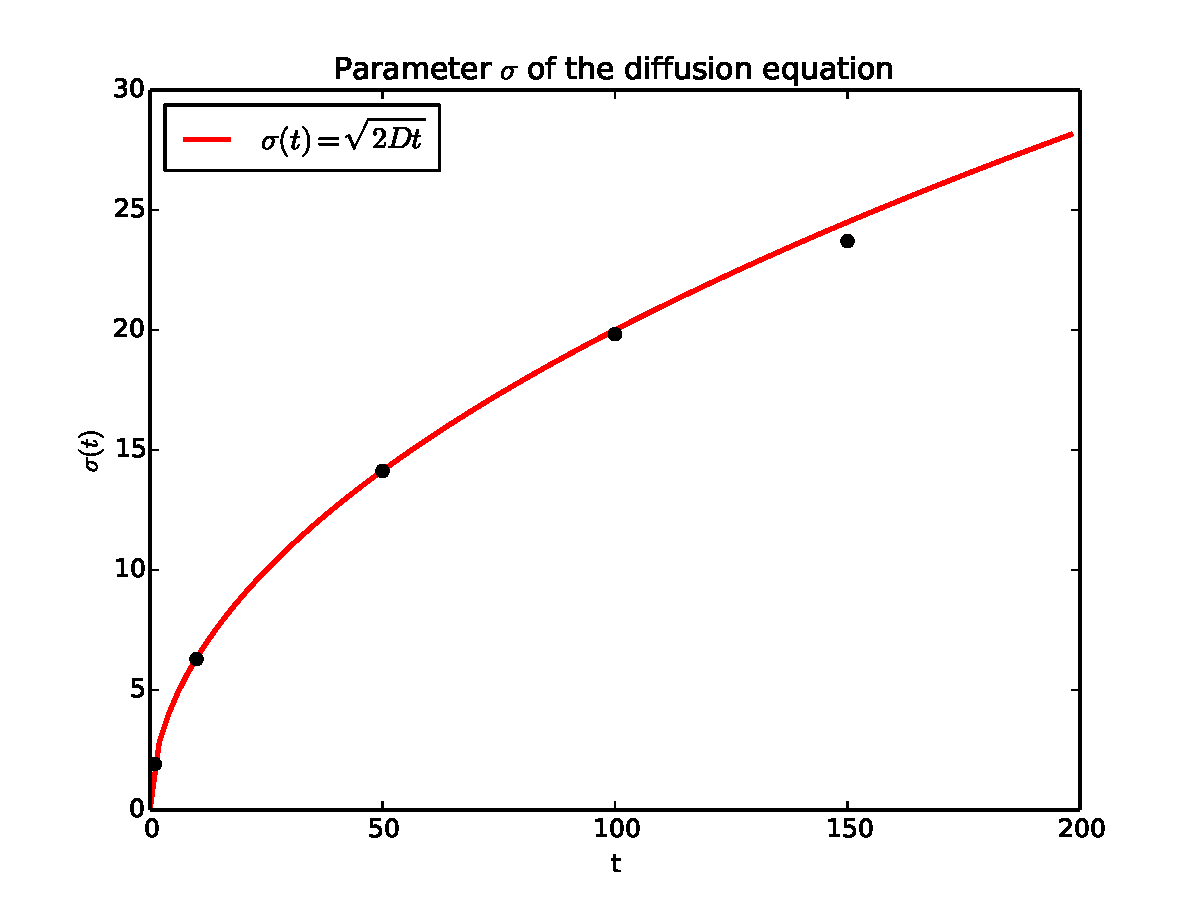
\includegraphics[width=10cm]{sigma.pdf}
\caption{$\sigma(t)$ versus time.}
\end{figure}
\begin{figure}[H]
\centering
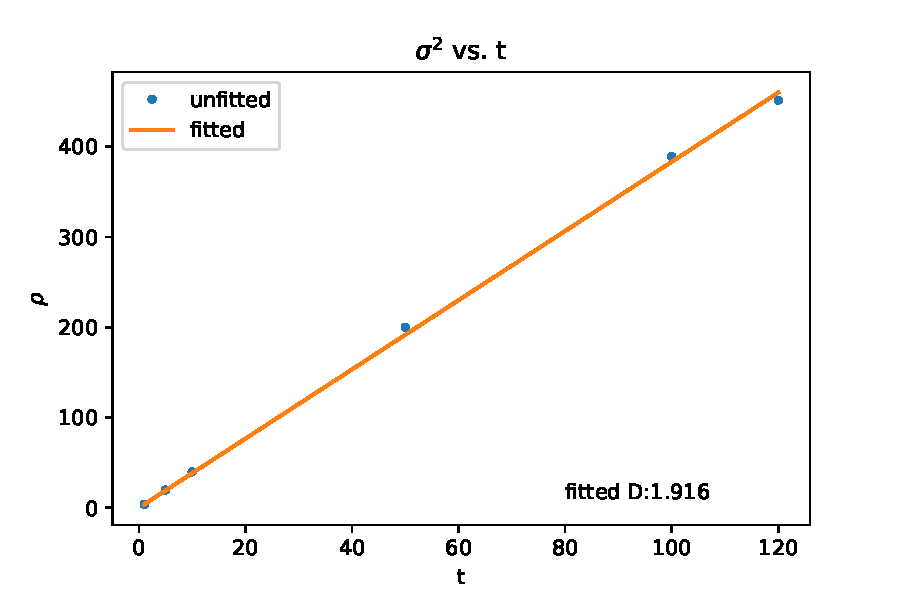
\includegraphics[width=10cm]{sigma2fit.pdf}
\caption{$\sigma^{2}(t) versus time.$}
\end{figure}
\noindent We observe that $\sigma(t)$ and $\sigma^{2}(t)$ follow the expected relationships with time, and that $D = 1.916$ for our fitted $\sigma^{2}(t)$ graph, which is a close value to our chosen $D = 2$.\par
\bigskip
\noindent 3. \textbf{Mixing of Two Gases}\par
\smallskip
Now we want to write a program that simulates the mixing of two gases in 2D in a rectangular enclosure. First, we set up a 2D grid with dimensions 120 x 80, and populate the left third of the grid with species "A", the right third of the grid with species "B", and leave the middle third of the grid empty. We pick a random location on the grid, and if it is occupied, we have the gas particle move at a random position up/down/left/right; if the selected neighbouring position is occupied, we reject the move and pick another particle. We repeat this for a large number of iterations. \par
In writing our program, there were three distinct attributes that allowed our algorithm to run in a timely manner. First, when picking a random location on the grid, we choose unoccupied sites rather than occupied sites. This is because there are twice as many occupied sites as unoccupied; choosing and checking whether each occupied site has an empty neighbour will take twice as long as choosing and checking whether an unoccupied site has an occupied neighour. So, we choose unoccupied sites; if it has an occupied neighbour, we move the gas particle to the unoccupied location. Second, we only generate one instead of two random integers, and use it both for choosing a random unoccupied site and choosing the direction of its neighbour. This is twice as fast as generating a random integer for choosing the unoccupied location, and then generating another random integer for choosing which direction the neighbour is. Last, we create a border of permanently occupied sites around the perimeter of the grid. This will always prevent a gas particle at the edge from moving outside the grid, but it allows us to sidestep checking the index of the gas particles, and having different instructions for particles at the edge of the grid. Without the if/else statements for edge particles, our algorithm can run significantly faster.\par
We make visual plots at different times to show the diffusion of gas A and gas B:\par
\begin{figure}[H]
\centering
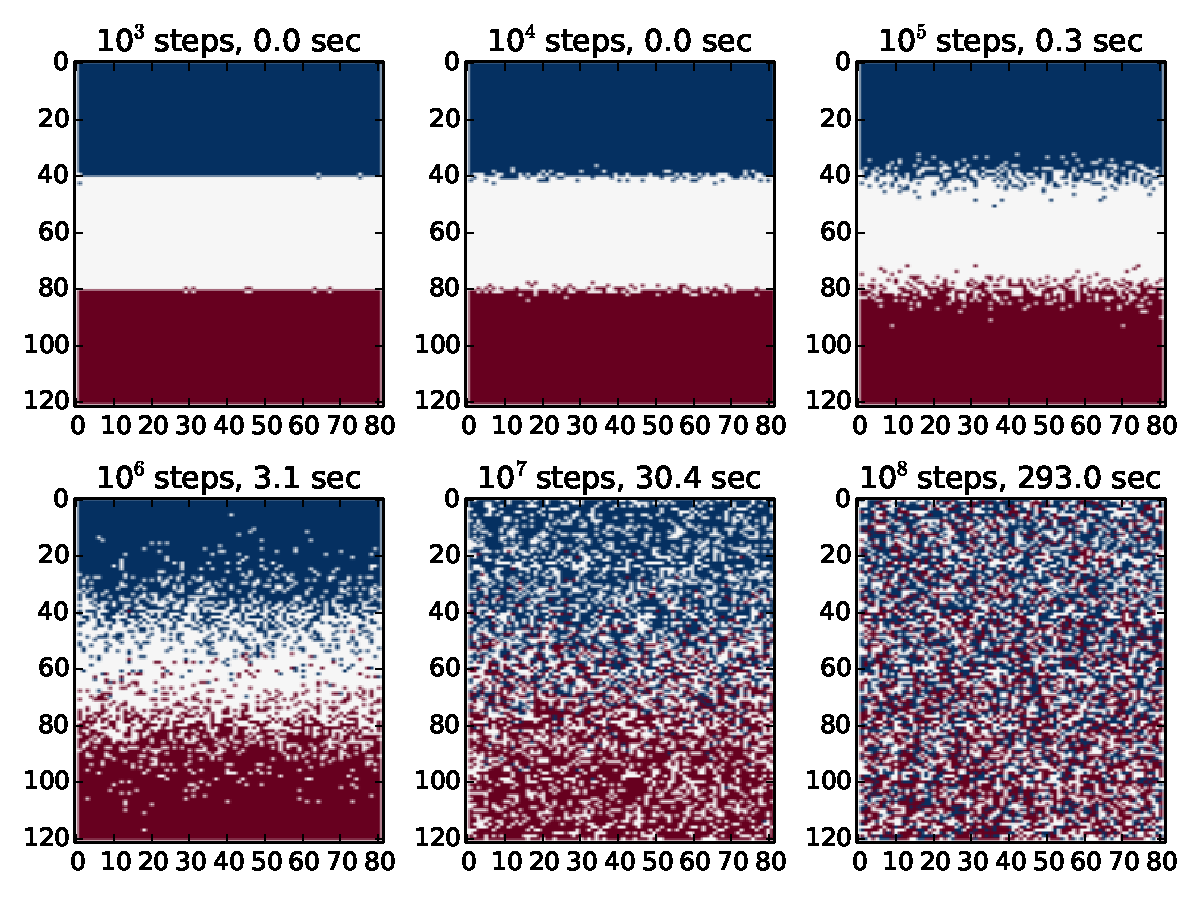
\includegraphics[width=12cm]{GP1_3b_1.pdf}
\caption{Sample configurations of grid with species A and species B at various times.}
\label{fig:grid}
\end{figure}
\noindent We see that species A and species B are mixing together more as time goes on, which is as expected. At 222.5 seconds, they seem to be almost completely mixed together, though from naked eye it seems that there is still a bit more blue on top, and a bit more red on the bottom. We note that it has taken 100 million steps to reach this point, and the two gases are still not entirely mixed together, although they are close. To reach "complete" mixing, we run the program for $10^{9}$ steps, or approximately 1600 seconds, and obtain Figure \ref{fig:maxdens}:\par
\begin{figure}[H]
\centering
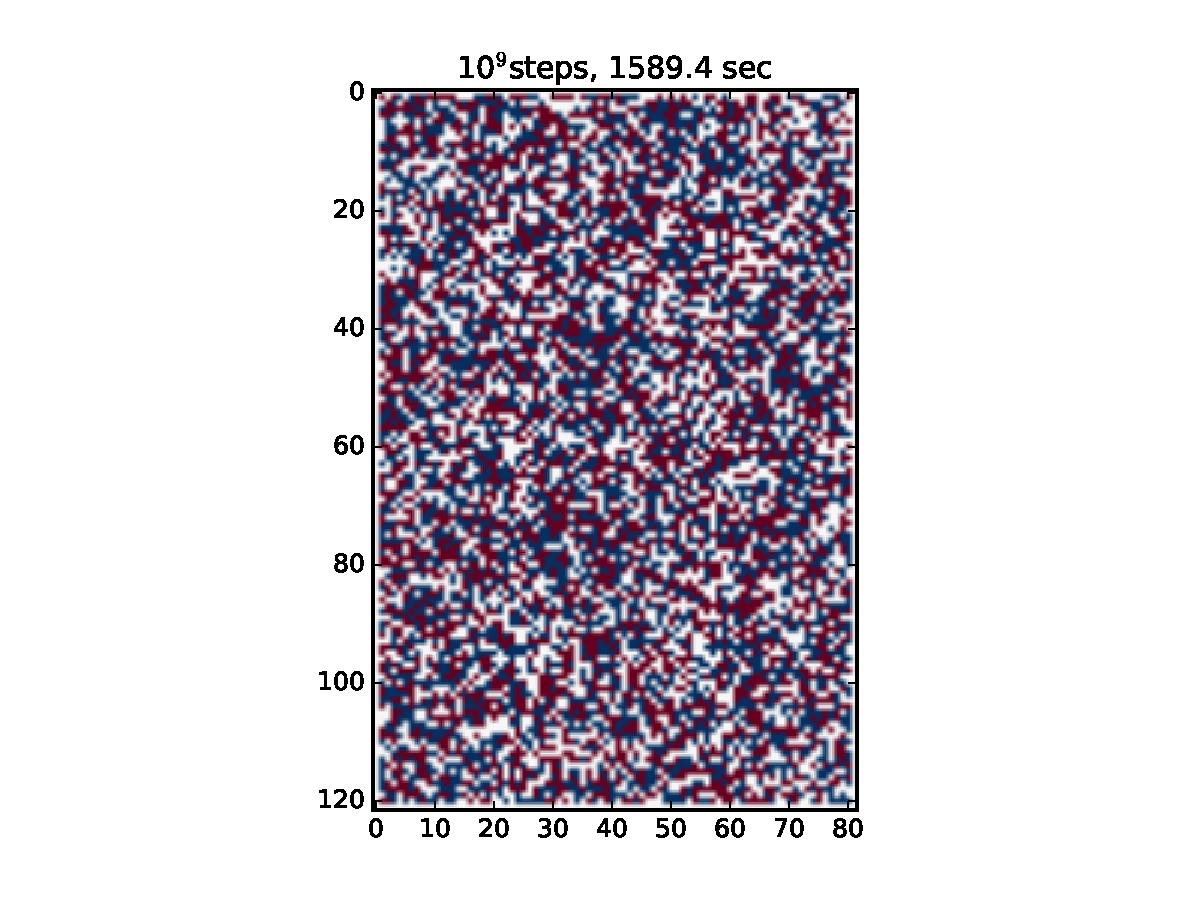
\includegraphics[width=12cm]{GP1_3_maxlimit.pdf}
\caption{Fully mixed gases A and B.}
\label{fig:maxdens}
\end{figure}
We also want to plot the linear population densities at the same time intervals to better visualize how separated the gases are.\par
\begin{figure}[H]
\centering
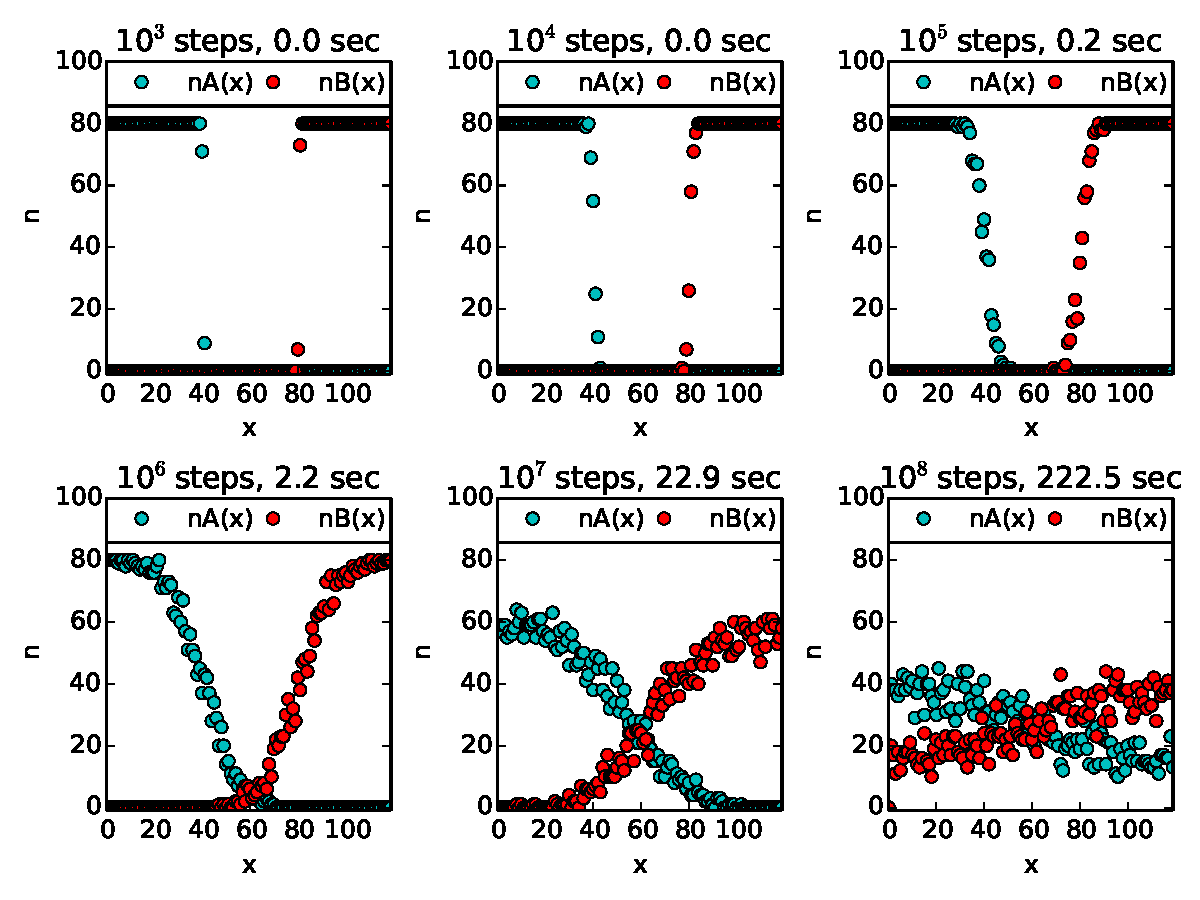
\includegraphics[width=12cm]{GP1_3b_2.pdf}
\caption{Linear population densities $n_{A}(x)$ and $n_{B}(x)$ at time intervals of Figure \ref{fig:grid}.}
\label{fig:dens}
\end{figure}

\noindent We see that, as expected, the linear population density of both species A and species B gradually decreases throughout time, with the decrease starting from the middle of the grid and making its way to the edges of the grid as time goes on. At 222.5 seconds, as we observed earlier, the two species are not completely mixed together; the linear population densities of species A and species B are still greater on the left and right sides of the grid, respectively. However, we note that viewing the linear densities of the species gives us a more accurate representation of how much each gas is diffused than simply looking at the grids in Figure \ref{fig:grid}. While we guessed using Figure \ref{fig:grid} above that the two gases were imperfectly mixed at 222.5 seconds, visualizing the unequally distributed linear densities allows us to say with more certainty that the two gases are still not fully mixed. Now, we can confirm our "complete" mixture in Figure \ref{fig:maxdens} by also plotting the linear densities:\par

\begin{figure}[H]
\centering
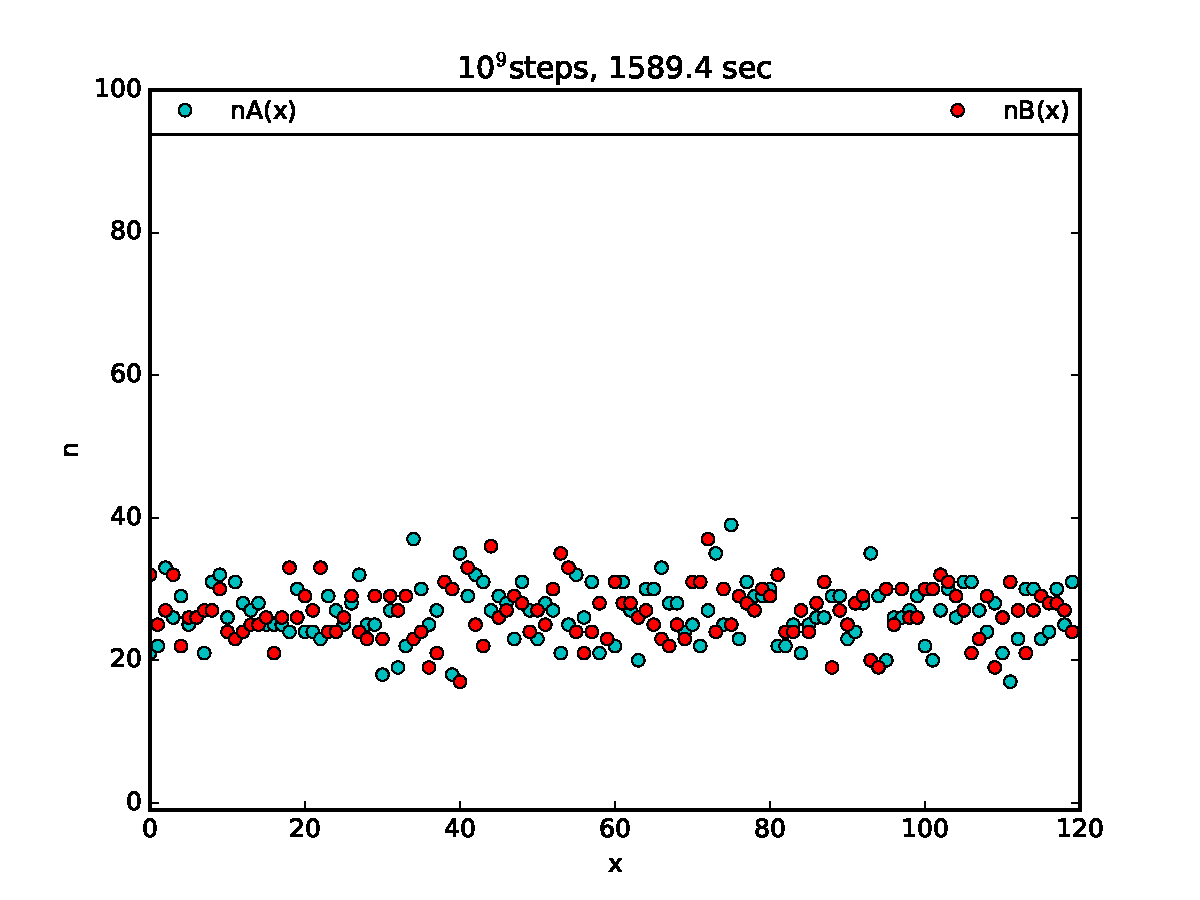
\includegraphics[width=10cm]{GP1_3_maxlimit_density.pdf}
\caption{Linear population density of fully mixed gases.}
\label{fig:maxdensplot}
\end{figure}

\noindent We can see that Figure \ref{fig:maxdensplot} shows an equal distribution of the linear population densities throughout the grid, unlike the last plot of Figure \ref{fig:dens}. Plotting the linear densities allows us to better determine how well-mixed the gases are.\par

Last, to increase our accuracy, we want to average the densities over 100 trials and replot the linear population densities. Figure \ref{fig:avgdens} shows this plot.\par

\begin{figure}[H]
\centering
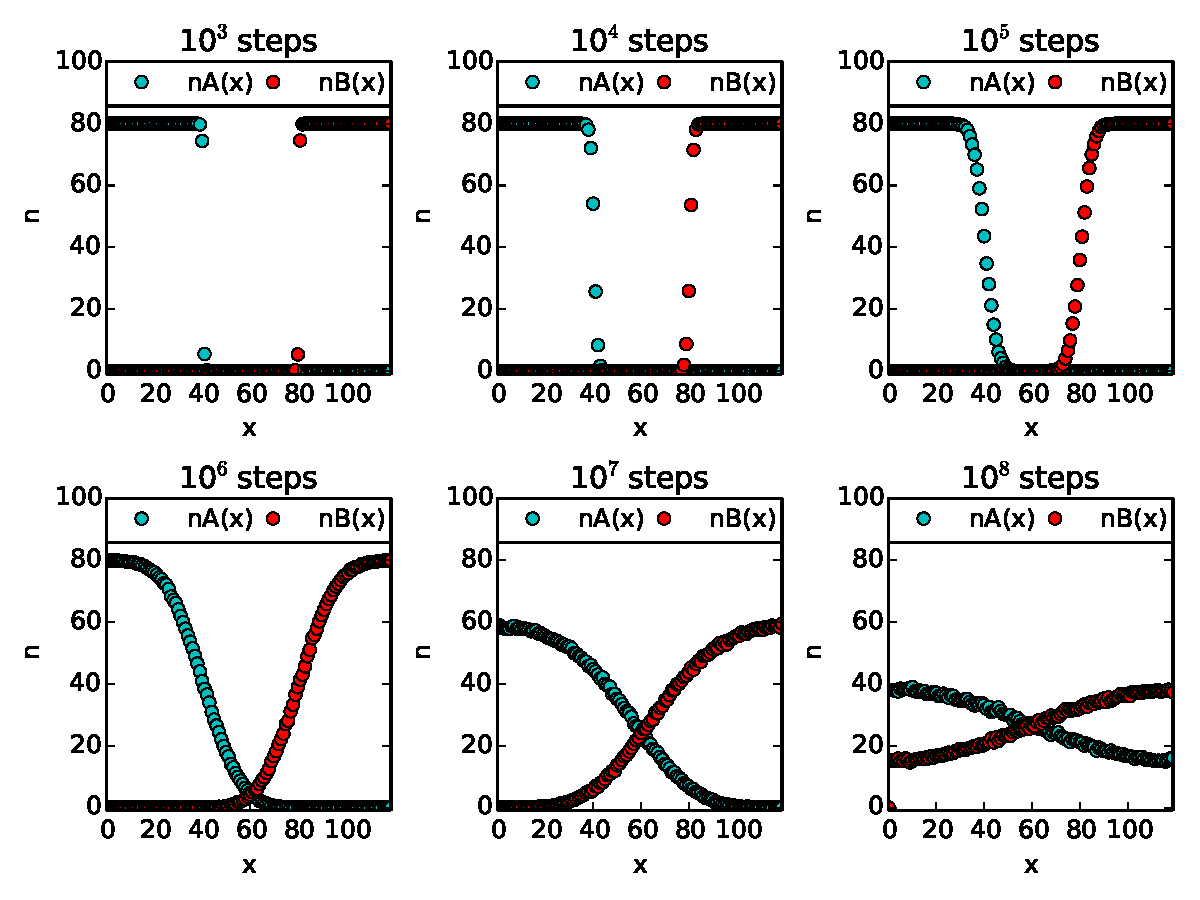
\includegraphics[width=12cm]{GP1_3c.pdf}
\caption{Linear population densities $n_{A}(x)$ and $n_{B}(x)$ at various number of steps, averaged over 100 trials.}
\label{fig:avgdens}
\end{figure}

\noindent Comparing Figures \ref{fig:dens} and \ref{fig:avgdens}, we observe that averaging over 100 trials makes the linear population density graphs more accurate and closely fit than just plotting over one trial. The individual points in Figure \ref{fig:avgdens} closely follow a clear fit, whereas the individual points in Figure \ref{fig:dens} are more scattered and deviate more from a single fit. This is as expected, as the more samples we have, the higher accuracy we expect out of our density plots.\par
\bigskip
\noindent GitHub repository: \url{https://github.com/LingfeiZhao/Group-Project-1b}
\end{document}

